\documentclass[12pt]{article}

\usepackage[margin=1in]{geometry}
\usepackage{graphicx}
\graphicspath{ {./images/class1/} }
\usepackage[x11names, dvipsnames]{xcolor}
\usepackage{minted}
\usepackage{gistex}
\usepackage{hyperref}
\usepackage[framemethod=tikz]{mdframed} % Allows defining custom boxed/framed environments

%----------------------------------------------------------------------------------------
%	INFORMATION ENVIRONMENT
%----------------------------------------------------------------------------------------
% Usage:
% \begin{info}[optional title, defaults to "Info:"]
% 	contents
% 	\end{info}

\mdfdefinestyle{info}{%
    topline=false, bottomline=false,
    leftline=false, rightline=false,
    nobreak,
    singleextra={%
        \fill[black](P-|O)circle[radius=0.4em];
        \node at(P-|O){\color{white}\scriptsize\bf T};
        \draw[very thick](P-|O)++(0,-0.8em)--(O);%--(O-|P);
    }
}

% Define a custom environment for information
\newenvironment{task}[1][Task:]{ % Set the default title to "Task:"
    \medskip
    \begin{mdframed}[style=info]
        \noindent{\textbf{#1}}
}{
    \end{mdframed}
}

\newenvironment{overview}
  {\noindent\rule{\textwidth}{0.4pt}
  \paragraph{Overview:}
  }
  {\par
  \noindent\rule{\textwidth}{0.4pt}
  }







\begin{document}
\raggedbottom
\setlength{\parskip}{0pt}

\title{CPEG472 Applied Cryptography}
\author{Andy Novicin}
\date{Spring 2019}

\maketitle

\section{Hello Crypto (A Brute force reverse-hash)}

\subsection{Introduction}
\begin{overview}
The next several katas (exercises) will have a series of tasks that walk you through the process of finding some dictionary word which has been hashed using only the result. In the process you will learn what a cryptographic hash function is, how to use codepen, cloud9, python, some great crypto libraries, basic command line scripting, and some basic coding. Most importantly you will begin to get a "gut-feel" for just how incredible modern CPUs are and why your human intuition for cryptography is not likely to be correct the first time you think about this stuff. Try to imagine the dictionary words as badly chosen passwords and think about how much "entropy" you need to make this attack infeasible.
\end{overview}

\paragraph{Peptalk:}
 This is not going to be easy, but if you stick it out you're going to have new super-powers. Every time you make progress you'll look back and wonder how you did it before. I am going to toss you into the deep-end of the pool and give you just a few google search terms to go with. Please don't get discouraged! When you are leading your team one day they will all look to you for the answers and you'll look to the internet for help. Mastery is not going to be immediate, but repeatable success will have to do. I could give you the resources to fill in all gaps but it would be large, possibly incomplete, and leave you less powerful than you would be hunting down success. I AM AVAILABLE TO HELP YOU WHERE YOU ARE THOUGH. Please don't hesitate to reach out directly.
 \newpage

\subsection{Kata: Hashing a dictionary word}

\begin{overview}
These two tasks will have you edit just a little bit of javascript code to get a "challenge word". If you succeed here you will have a hashed word from a standard dictionary. The next kata's will walk you through finding which word was hashed to get your word.par
\end{overview}

In this course I want you to be an effective wielder of cryptography. That means knowing how to use strong crypto schemes and knowing how to attack a weak scheme.\\

So we're going to begin by attacking SHA-512. Muah-ha-ha-ha. (You don't know what this stuff means yet but this is a top-of-the-line "Hash function". Play with this next snippet and things will start to make some sense.)

\begin{task}[CodePen 101 Task:]
Use the below codepen sample to ask my server for a random word from the scrabble dictionary to be hashed with SHA512. Now hash your own word using the input box to check that the crypto.js library's SHA512 matches PHP's SHA512 hash. (I know we haven't discussed what this means yet.)
\end{task}

There is supposed to a JS thing here\\

So you might now have some intuition that a "hash function" can create a long nasty looking string of letters and numbers. Also that you can feed the hash a word and get the same nasty looking string of letters and numbers. You've intuitively picked up that the hash is a repeatable scrambler of some input.

%\begin{task}[CodePen 102 Task:]
% Now edit the JavaScript of that pen. Change the source of the XHR request from https://vip.udel.edu/crypto/sha512_with_answer.php to https://vip.udel.edu/crypto/sha512.php . (Look for that first URL and remove "_with_answer".) This gives you the "hash" without telling you what word created it. Try a few random words that you think up on your own to see if you can find a match by just chance.
% \end{task}

 Now you know the main challenge of this lesson: A random word has been hashed with a strong hash function and we are trying to figure out which word it was. In the process we're going to pick up some subtle lessons about how to think in modern cryptographic terms.

\begin{overview}
This section has no action steps for you to take, it is solely here to help explain the basics of a cryptographic hash function. We will be talking more about hash functions later in the course so you don't have to know this too deeply yet. But I want to have you code sooner rather than have to wait weeks before you're brave enough. So this section is just enough that you don't stress out when you start actually coding.
\end{overview}

Now that you know the mini-challenge of lesson 1 let me tell you a bit about hash functions.\\

A hash function is something which creates a type of fingerprint from a string (or any sequence of bits). Every time anyone runs the same hash function on the same input they should get the same output.\\

Hash functions take in arbitrary length input and spit out a fixed-length output.\\

Hash functions are used as part of digital signatures, "checksums", in Message Authentication Codes (MACs), and in password storage. We'll talk about all of these thing in detail as we progress through this course. For now here are the properties of a good hash function:\\

    Hash functions do not use a key. A key is a secret bit of information which let's you decrypt some encrypted message. In the case of hash functions it should be pretty much impossible to "decrypt"/"reverse" a hash.\\
    Crytographic hash functions should be hard to invert. That is, given h(s) but not s, it should be computationally expensive to find s.\\

Hash functions should be fast to compute.\\

Given an input and the hash of that input, it should be hard to compute a second message which hashes to the same value. That is, given x1,h(x1) it should be hard to compute x2 such that h(x1)==h(x2).\\

    It should be hard to find any two inputs that hash to the same thing.\\

SHA-512 is from the 2nd round of "Secure Hash Algorithms" and the output is always 512-bits. It is the most secure hash out there, although there is a 3rd iteration (SHA-3) which has just been finalized as of late 2015.\\

\section{Fire up a workspace/CPU on Cloud9 or Code Anywhere}

\begin{overview}
This kata is aimed at getting you up to speed with tools that I intend to have you use on a daily basis during this course. Cloud9 is a great tool for having your own machine that you can code and command as you see fit. I also think it's valuable to have you learn command-line linux which will happen as a side-effect of working through these katas. When you are done with this kata you should have put a secret hashed word into a textfile on a new virtual machine that you control, all in your standard web browser (I prefer Chrome for this). For this course I'm going to have you do most of the heavy lifting in a scripting language. JavaScript, Python, or PHP will all fit the bill, you don't have to know those languages right now. In the next kata we will explore basic crypto in Python.
\end{overview}

Cloud9 will be a full powered development environment that we use to script/code/hack/server right in the browser.

\begin{task}[Login to Github]
If you don't have a GitHub account, go make one now.
\end{task}

\begin{task}[Cloud9 Task:]
Cloud9 Task: You should have an email invite to cloud9 (maybe in your spam box). Now head to https://c9.io FOLLOW THE LINK FOR USERS OF THE PREVIOUS c9.io (NOT AWS) and use your github account to create a Cloud9 account. It will say the TEAM IS FULL, ignore that and click dashboard in the top right.
\end{task}

Cloud9 is a wonderful place where you can spawn up your own servers each running a well equipped Ubuntu.

\begin{task}[Create a workspace:]
Create a workspace: Spawn a workspace, name it something like sha512 , and make it a "Python"-type workspace. I've added some screenshots to help:
\end{task}

\gistex{https://gist.github.com/dc83b8d8d189b46cce7e.git}

\begin{center}
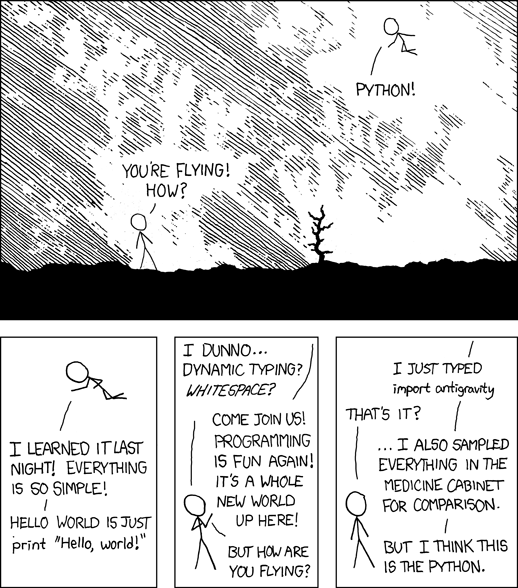
\includegraphics[scale=.5]{python}
\end{center}

\end{document}
